\documentclass[2pt]{article}
\usepackage{amsmath,amsthm,amssymb,geometry,graphicx,wrapfig,commath}
\usepackage[font={small,it}]{caption}
\usepackage{url}
\title{\textbf{Harmonic Number}}

\begin{document}
\date{\vspace{-5ex}}
\maketitle 
\section{Introduction}
\begin{wrapfigure}{r}{8cm}
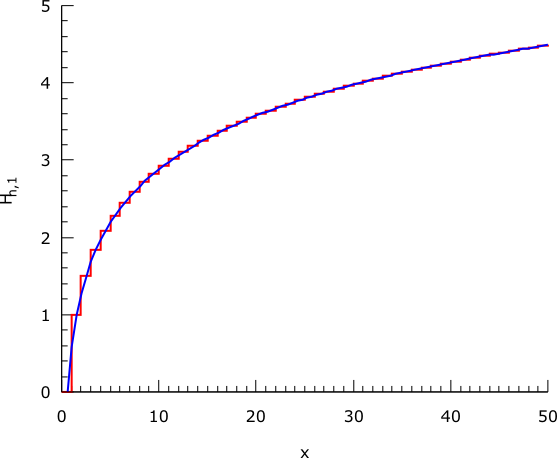
\includegraphics[width=8cm]{1.png}\caption{\small{The harmonic number $H_{n,1}$ with $n=\lfloor{x}\rfloor$ (red line) with its asymptotic limit $\gamma+\ln(x)$ (blue line).}}\end{wrapfigure}
\begin{flushleft}
The term \emph{Harmonic number} has multiple meanings.
\end{flushleft}
In mathematics, the n-th harmonic number is the sum of the reciprocals of the first n natural numbers:
\begin{equation}
H_{n}=1+\frac{1}{2}+\frac{1}{3}+...+\frac{1}{n}=\sum_{i=1}^n \frac{1}{n} \label{nth harmonic number}\nonumber
\end{equation}

\par This also equals n times the inverse of the \emph{harmonic mean} of these natural numbers.\\
\par Harmonic numbers were studied in antiquity and are important in various branches of number theory. They are sometimes loosely termed harmonic series, are closely related to the Riemann zeta function, and appear in the expressions of various special functions.\\
\par The associated harmonic series grows without limit, albeit very slowly, roughly approaching the natural logarithm function. 
\par In 1737, Leonhard Euler used the divergence of this series to provide a new proof of the infinity of prime numbers. His work was extended into the complex plane by Bernhard Riemann in 1859, leading directly to the celebrated Riemann hypothesis about the distribution of prime numbers.\\
\par When the value of a large quantity of items has a Zipf's law distribution, the total value of the n most-valuable items is the n-th harmonic number. This leads to a variety of surprising conclusions in the Long Tail and the theory of network value.\\
\par Bertrand's postulate entails that, except for the case n=1, the harmonic numbers are never integers.
\\
\section{Identities involving harmonic numbers}
By definition, the harmonic numbers satisfy the \emph{recurrence relation}
\begin{equation} 
H_{n}=H_{n-1}+\frac{1}{n} \label{recurrence relation}\nonumber
\end{equation}
They also satisfy the series Identity
\begin{equation}
\sum_{k=1}^n H_{k} = (n+1) H_{n} - n \label{Series Identity}\nonumber
\end{equation}
The Harmonic numbers are connected the \emph{Stirling Numbers} of first kind
\begin{equation}
H_{n} = \frac{1}{n!} {n+1 \choose 2} \label{Stirling Identity}\nonumber
\end{equation}
The functions
\begin{equation}
f_{n} (x) = \frac{x^n}{n!} (\log{x}-H_{n})\nonumber
\end{equation}
satisfy the property
\begin{equation}
{f'}_{n} (x) = f_{n-1} (x)\nonumber
\end{equation}
In particular
\begin{equation}
f_{1} (x) = x(\log{x}-1)   \nonumber    			
\end{equation}

\section{Eulerian Representation}
An integral representation is given by
\begin{equation}
H_{n} = \int_{0}^{1} \frac{1-x^n}{1-x} dx \label{Euler equation}\nonumber
\end{equation}
The equality above is obvious by simple algebraic identity
\begin{equation}
\frac{1-x^n}{1-x} = 1+x+...+x^{n-1}\nonumber
\end{equation}
Using a simple integral transform ${x = 1-u}$, an elegant combinatorial expression for $H_{n}$ is\\
\begin{align}
H_{n} &= \int_{0}^{1} \frac{1-x^n}{1-x} dx\nonumber \\
	 &= -\int_{1}^{0} \frac{1-{(1-u)}^n}{u} dx \nonumber \\
	 &= \int_{0}^{1} \frac{1-{(1-u)}^n}{u} dx \nonumber \\
	 &= \int_{0}^{1} \bigg{[}\sum_{k=1}^{n} (-1)^{k-1} {n \choose k} u^{k-1}\bigg{]}dx \nonumber \\
	 &= \sum_{k=1}^{n} (-1)^{k-1} {n \choose k} \int_{0}^{1} u^{k-1} \nonumber dx\\
	 &= \sum_{k=1}^{n} (-1)^{k-1} \frac{1}{k} {n \choose k} \nonumber
\end{align}
The same representation can be produced by using the third \emph{Retkes Identity} by setting $x_{1} = 1, . . . , x_{n} = n$ and using the fact that
\begin{equation}
{\Pi}_{k}(1, . . . , n) = {(-1)}^{n-k} (k-1)!(n-k)! \nonumber
\end{equation}
\\
\begin{equation}
H_{n}=H_{n,1}=\sum_{k=1}^{n} \frac{1}{k} = {(-1)}^{n-1}n!\sum_{k=1}^{n}\frac{1}{k^{2}{\Pi}_{k}(1, . . . ,n)}=\sum_{k=1}^{n}{(-1)}^{k-1}\frac{1}{k}{n \choose k} \nonumber
\end{equation}
\\
\section{Approximation of $H_{n}$ by $\int_{0}^{1}\frac{1}{x} dx$}
\begin{wrapfigure}{r}{6cm}
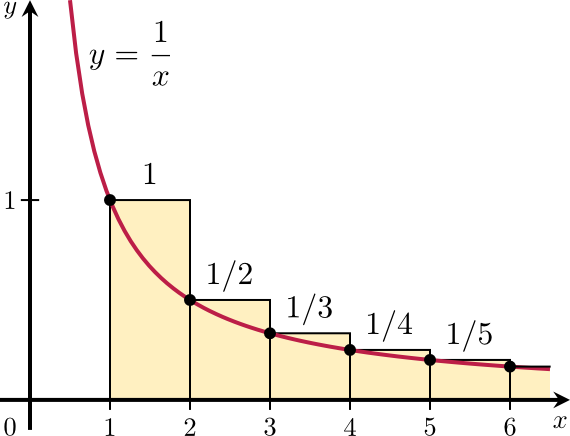
\includegraphics[width=6cm]{2.png}
\caption{\small{Graph demonstrating a connection between harmonic numbers and the natural logarithm. The harmonic number $H_{n}$ can be interpreted as a Riemann sum of the integral: $\int_1^{n+1} \frac{1}{x} \mathrm{d}x = \ln(n+1)$}}
\end{wrapfigure}

The harmonic sum is the sum of reciprocals of the positive integers.
\\
We have
\begin{equation}
\frac{1}{n} < \int_{n-1}^{n} \frac{dt}{t} , n \geq 2\nonumber
\end{equation}
\begin{equation}
\frac{1}{n} > \int_{n}^{n+1} \frac{dt}{t} , n \geq 1\nonumber
\end{equation}
Hence we can say, by a summation of $n$ upto $N$

\begin{equation}
\int_{1}^{N+1} \frac{dt}{t} < \sum_{n=1}^{N} \frac{1}{n} < 1 + \int_{1}^{N} \frac{dt}{t}\nonumber
\end{equation}
\pagebreak
\begin{equation}
\log{(N+1)} < \sum_{n=1}^{N} \frac{1}{n} < 1 + \log{N}\nonumber
\end{equation}
since $\log{N} < \log{(N+1)}$ we can write\\
\begin{equation}
\log{N} < \sum_{n=1}^{N} \frac{1}{n} < 1 + \log{N}\nonumber
\end{equation}
Now we can further write
\begin{equation}
\sum_{n=1}^{N} \frac{1}{n} = \log{N} + O(1)\nonumber
\end{equation}
Hence we can introduce some constant $\lambda < 1$ such that
\begin{equation}
\abs{\sum_{n=1}^{N} \frac{1}{n} - \log{N}} \leq \lambda , \forall N\nonumber
\end{equation}
The $n^{th}$ harmonic number is about as large as the \emph{natural logarithm} of $n$. The reason is that the sum is approxiamted by the integral
\begin{equation}
\int_{1}^{n} \frac{1}{x} dx\nonumber
\end{equation}
whose value is \emph{ln(n)} \\
\\
Can we get any better?This is all wonderful, but can we do better? That is, can we be more precise about the
error. \\ Lets see, begin with
\begin{equation}
a_{n} = \frac{1}{n}-\int_{n}^{n+1}\frac{dt}{t} \nonumber
\end{equation}
Integrating it and using properties of logarithm
\begin{equation}
a_{n}=\frac{1}{n}-log{(1+\frac{1}{n})}
\end{equation}
and expanding via the Taylor series for $\log{(1 + x)}$ which converges for $-1 \leq x \leq 1$, we get
\begin{equation}
a_{n} = \frac{1}{n} - \bigg{(}\frac{1}{n} -\frac{1}{2n^2}+\frac{1}{3n^3}...\bigg{)}=\frac{1}{2n^2}-\frac{1}{3n^3}
\end{equation}
This is an alternating series where terms decrease in absolute value, so we see that
\begin{equation}
0<a_n<\frac{1}{2n^2}
\end{equation}
A consequence of this inequality is that the sum 
\begin{equation}
\sum_{n=1}^{\infty} a_n
\end{equation}
is a constant. Call this constant $\gamma$. Now we can say that
\\\\
The values of the sequence $H_{n} - ln(n)$ decreases monotonically towards the \emph{limit}
\begin{equation}
\lim_{n \to \infty} (H_{n} - ln(n)) = \gamma\nonumber
\end{equation}
where $\gamma \sim 0.5772156649$ is the \emph{Euler-Mascheroni Constant}. The correspondng \emph{asymptotic expansion} as $n \to \infty$ is
\begin{equation}
H_{n} \sim ln \emph{n} + \gamma + \frac{1}{2n}-\sum_{k=1}^{\infty} \frac{B_{2k}}{skn^{2k}}=ln \emph{n} + \gamma + \frac{1}{2n} - \frac{1}{12n^2}+\frac{1}{120n^4}-...\nonumber
\end{equation}
where $B_{k}$ are the \emph{Bernoulli Numbers}.

\nocite{*}
\bibliography{mybib.bib}{}
\bibliographystyle{plain}
\end{document}













